
\subsection{Laser positioning system}
\label{sec:calib-laser-pos}

Because the precision of the \efield measurement relies heavily on a precise knowledge of the laser beam tracks, an independent measurement of their direction for some specific positions is required. The laser positioning system addresses this requirement.
%\subsubsection{Physics Motivation}
While the direction of the laser beam will be very well known based on the reading from the encoders on the laser beam steering mechanism,  residual uncertainty or unpredictable shift in the pointing direction will remain. 
%Having 
Keeping in mind the long length of the ionization track of more than \SI{15}{\m}, even a small offset in the pointing direction can lead to vastly different ionization track locations, especially close to the end of the track. Such inaccuracies will directly affect our ability to precisely calibrate any variations in the \efield.

\subsubsection{Design}

The laser positioning system (LPS) \fixme{LPS is not in the common glossary.} is designed to address the problem of precise and accurate knowledge of the laser track coordinates. %University of Hawaii group has 
Two complementary systems are planned, one based on PIN diodes and another based on mirrors.

\paragraph{Pin-diode system for laser positioning}

A system based on PIN \fixme{PIN is also not in the common glossary.}diodes 
%(consisting of 1$\times$3) array 
was built for the mini\dword{captain} experiment, \fixme{needs ref} and the installed version is visible in the photograph of the mini\dword{captain} \dword{tpc} as shown in  Figure~\ref{fig:LPS_miniCAPTAINlabeled}.  

%\begin{figure}[htb!] 
%\centering 
%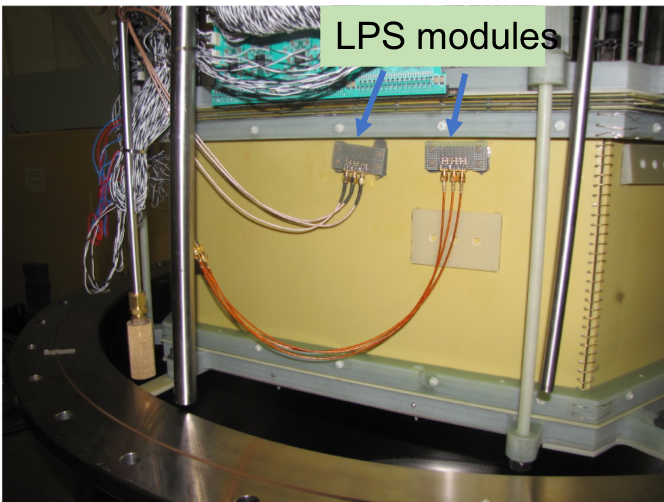
\includegraphics[width=0.6\linewidth]{LPS_miniCAPTAINlabeled.png} 
%\caption{Photo of the miniCAPTAIN TPC with two LPS modules glued on the outside to detect laser beam spot location via fluorescence of the TPC FR4 wall when illuminated by the laser beam.}
%\label{fig:miniCAPTAIN} 
%\end{figure}

\begin{dunefigure}[Laser positioning system modules in the miniCAPTAIN TPC]{fig:LPS_miniCAPTAINlabeled}
{Photograph of the miniCAPTAIN TPC with two LPS modules glued on the outside to detect laser beam spot location via fluorescence of the TPC FR4 wall when illuminated by the laser beam.}
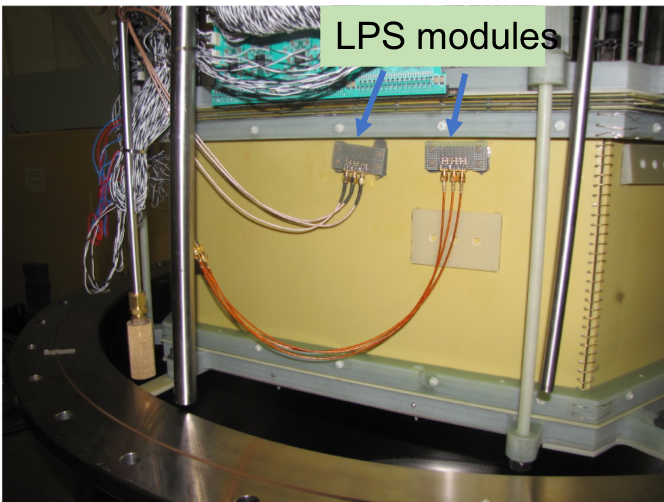
\includegraphics[width=0.6\linewidth]{LPS_miniCAPTAINlabeled} 
\end{dunefigure}

The LPS consists of groups of \num{9} PIN diodes, operating in passive, photovoltaic mode. These are GaP diodes with a sensitivity range extending down to  \SI{200}{\nano\m} wavelength; thus, detecting \SI{266}{\nano\m} light is straightforward. Figure~\ref{fig:GaP_diode_room_temp} shows signal detected at room and cryogenic temperatures. PIN diode is illuminated by the \SI{266}{\nano\m} light from the Nd:Yag
laser in the laboratory 
%(in the lab at University of Hawaii) 
set at lowest possible setting for minimal power.  \fixme{add lps to gloss}

PIN diodes are placed at the bottom of the cryostat and receive light passing through the gaps between the \dword{fc} profiles to minimize interference with the \dword{fc}. Drawings of one such group of PIN diodes are shown in Figure~\ref{fig:GaP_assembly}. With the group of \num{9} photodiodes, we can detect not only the beam but also crudely characterize its profile, giving a more precise location of the central beam pulse axis.


%\begin{figure}[htb!] 
%\begin{minipage}[b]{0.47\textwidth}
%\centering 
%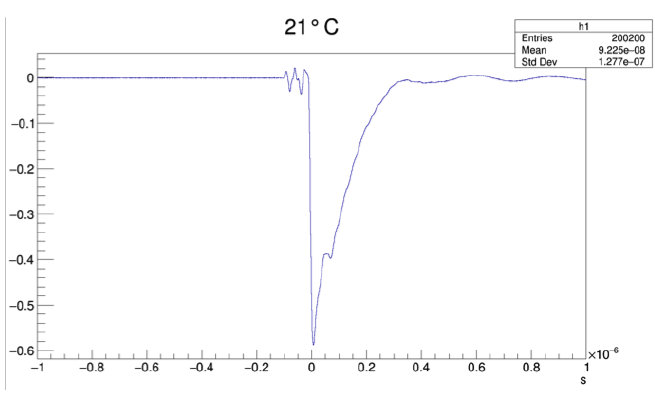
\includegraphics[width=0.95\linewidth]{GaP_diode_room_temp.png} 
%\caption{Signal from the GaP pin diode. The signal was a result of illumination of the PIN diode face with a 266\,nm laser at room temperature.}
%\label{fig:LPS1} 
%\end{figure}
%\end{minipage}
%\hfill
%\begin{minipage}[b]{0.47\textwidth}
%\begin{figure}[htb!] 
%\centering 
%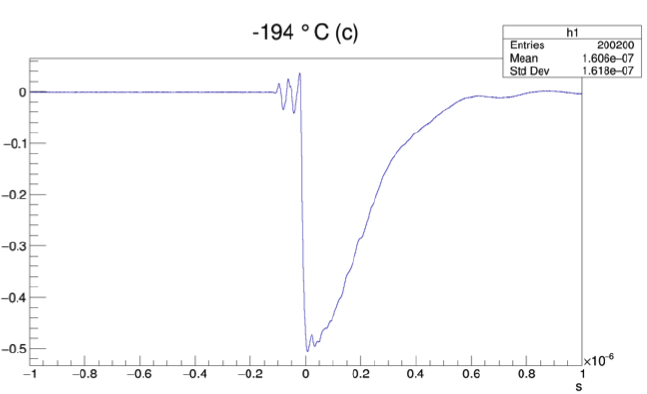
\includegraphics[width=0.95\linewidth]{GaP_diode_cryo_temp.png} 
%\caption{Signal from the GaP pin diode. The signal was result of illumination of the PIN diode face with a 266\,nm laser at cryogenic temperature.}
%\label{fig:LPS2} 
%\end{minipage}
%\hfill
%\end{figure} 


%\begin{figure}[htb!] 
%\begin{minipage}[b]{0.47\textwidth}
%\centering 
%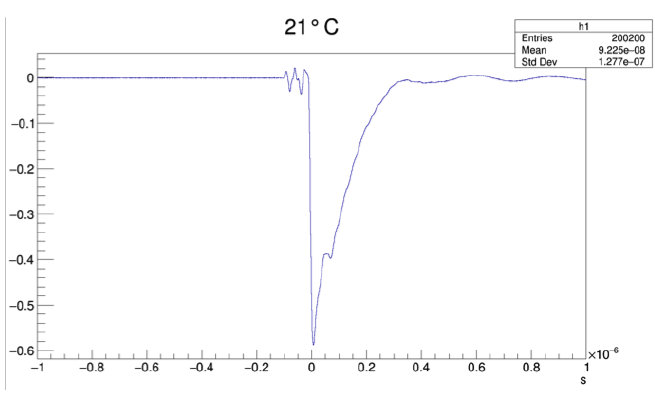
\includegraphics[width=1.0\linewidth]{GaP_diode_room_temp.png} 
%\caption{Signal from the GaP pin diode. The signal was a result of illumination of the PIN diode face with a 266\,nm laser at room temperature.}
%\label{fig:LPS1} 
%\end{minipage}
%\hfill
%\begin{minipage}[b]{0.47\textwidth}
%\centering 
%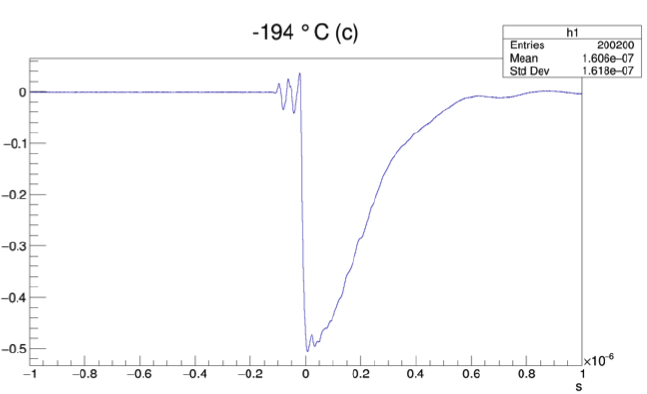
\includegraphics[width=1.0\linewidth]{GaP_diode_cryo_temp.png} 
%\caption{Signal from the GaP pin diode. The signal was result of illumination of the PIN diode face with a 266\,nm laser at cryogenic temperature.}
%\label{fig:LPS2} 
%\end{minipage}
%\hfill
%\end{figure} 


\begin{dunefigure}[Signal from the miniCAPTAIN laser positioning system at room and cryogenic temperatures]{fig:GaP_diode_room_temp}
{Signal from the miniCAPTAIN laser positioning system GaP PIN diode. The signal is a result of illumination of the PIN diode face with a \SI{266}{\nano\m} laser at room (left) and cryogenic (right) temperatures.}
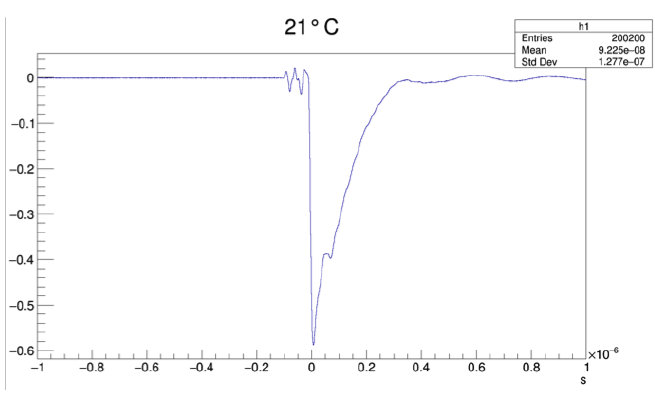
\includegraphics[width=0.47\linewidth]{GaP_diode_room_temp.png} 
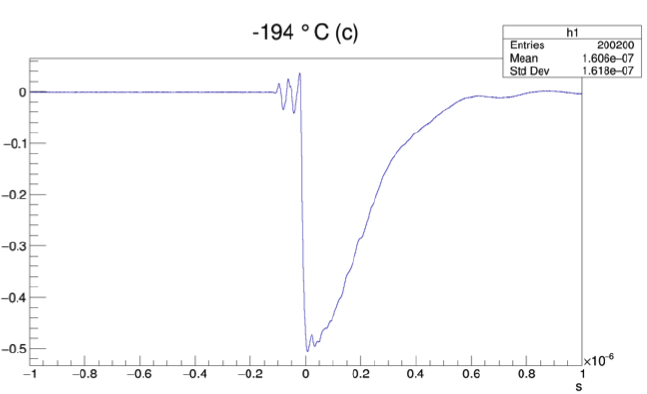
\includegraphics[width=0.47\linewidth]{GaP_diode_cryo_temp.png} 
\end{dunefigure}



\begin{dunefigure}[Cluster assembly of the miniCAPTAIN laser positioning system]{fig:GaP_assembly}
{(Left) LPS cluster mounted on the opposite wall from the laser periscope to detect and accurately determine the end point of the laser beam. (Right)
Profile of the LPS group mounted on the PCB. GaP diodes come with pins that use pair of twisted wires to transport the signal.
}
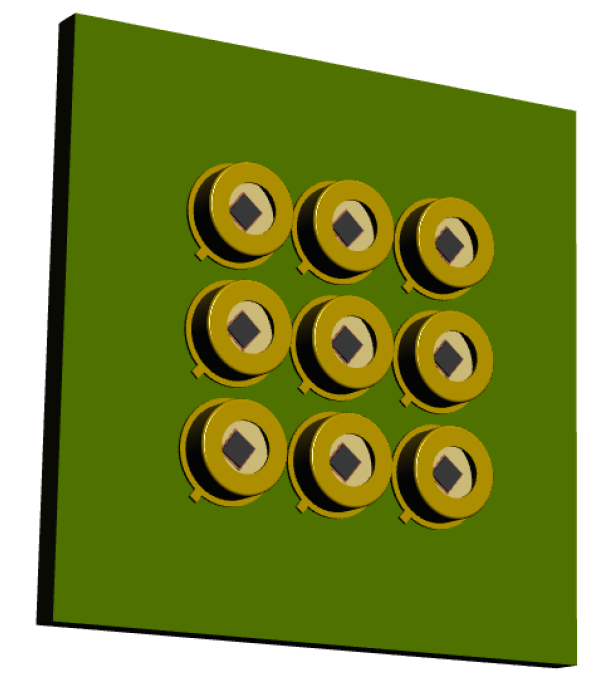
\includegraphics[width=0.47\linewidth]{GaP_assembly.png} 
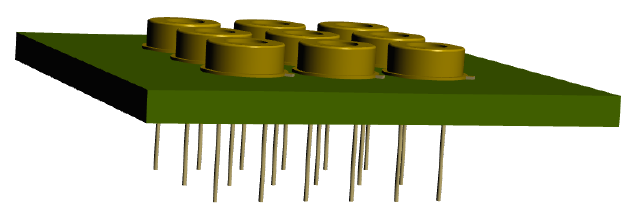
\includegraphics[width=0.47\linewidth]{GaP_assembly_profile.png} 
\end{dunefigure}


There will be one LPS pad per laser. The laser should always send the first pulse in the direction of the LPS before proceeding into a calibration sequence. 
%The electronics used to collect signals from the LPS will be provided by \dword{cisc}.\todo{CISC doesn't provide electronics. SG emails Jelena to clarify this.}


\paragraph{Mirror-based beam positioning system:}

In addition to the pin-diode system, we will also have clusters of small mirrors that allow measuring the beam end position via its reflections.

Figure~\ref{fig:laser_mirror_positioning} shows a conceptual sketch with a cluster of 6 mirrors located close to each other, but with different angles. When the beam hits one of the mirrors, it will be reflected back into the \dword{tpc}, and the reflection angle unambiguously identifies which mirror was actually hit. With small mirrors, \SI{5}{\milli\m} in diameter, the required positioning precision would be met if these mirrors are placed at distances of more than \SI{10}{\m}. The preferred location is, therefore, at the bottom \dword{fc}. Because the cluster can be small (a few cm), it can fit inside the \dword{fc} profiles. For each drift volume segment seen by two lasers, we plan to install at least two clusters, for redundancy, so the total number of clusters would be \num{32}. 

The simplest solution would be to use polished aluminum as the reflecting surface, so that the cluster could be a single block. Tests must be done for the actual reflectivity of the (oxidized) surface. An alternative could be using small dielectric mirrors.

\begin{dunefigure}[Mirror-based laser beam positioning system]{fig:laser_mirror_positioning}
{View of the mirror cluster for the beam positioning system inserted in the \dword{fc} profiles~\cite{bib:yu2019a}.}
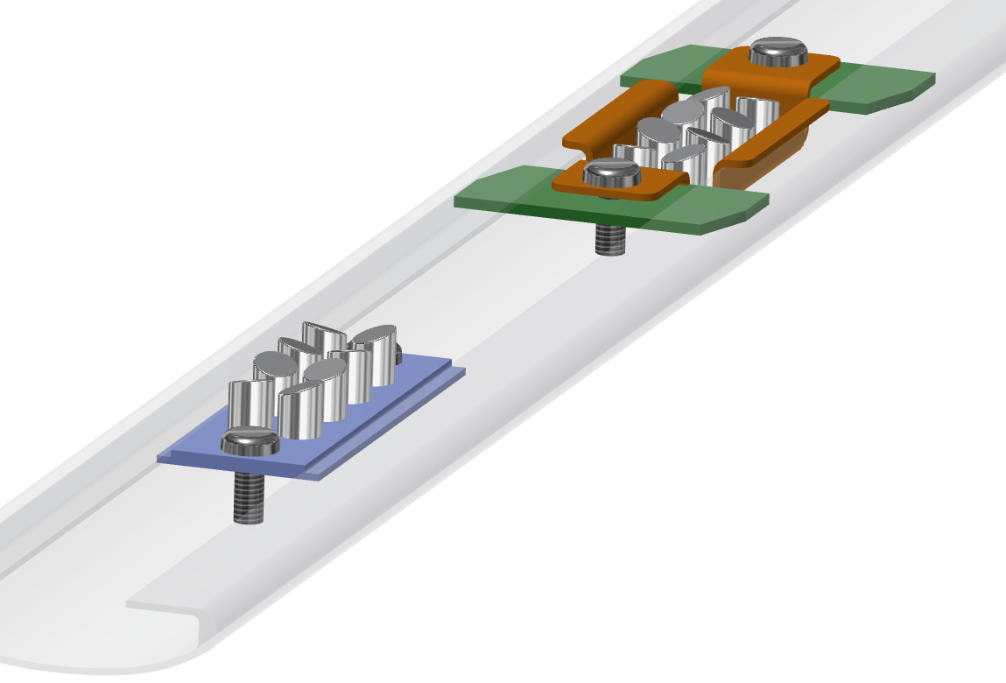
\includegraphics[width=0.7\linewidth]{laser_mirror_positioning.pdf}
\end{dunefigure}

\fixme{Nora stopped here.}

\subsubsection{Development plan}
 Further optimization of the LPS assembly to reduce electronic noise and cross-talk is required. Also, the size and shape of the cluster that would best collect the light coming through the field cage gaps needs to be optimized.  Another important aspect is durability of the system that will require extensive running in the cryogenic conditions with  a large number of cool-downs to validate GaP for extended use in DUNE. Finally, alternatives to GaP diodes such as SiPMs are under consideration. While SiPMs require power, their sensitivity to single photons makes them a desirable candidate for low light signals and more accurate beam direction reconstruction. 
















